%%%%%%%%%%%%%%%%%%%%%%%%%%%%%%%%%%%%%%%%%%%%%%%%%%%%%%%%%%%%
%%% ELIFE ARTICLE TEMPLATE
%%%%%%%%%%%%%%%%%%%%%%%%%%%%%%%%%%%%%%%%%%%%%%%%%%%%%%%%%%%%
%%% PREAMBLE 
\documentclass[9pt,lineno]{elife}
\usepackage[colorlinks=true]{hyperref}
% Use the onehalfspacing option for 1.5 line spacing
% Use the doublespacing option for 2.0 line spacing
% Please note that these options may affect formatting.

\usepackage{lipsum} % Required to insert dummy text
\usepackage[flushleft]{threeparttable}
\usepackage[version=4]{mhchem}
\usepackage[group-separator={,}]{siunitx}
\DeclareSIUnit\Molar{M}
\usepackage{newfloat}
\DeclareFloatingEnvironment[name={Box}]{codebox}
\usepackage[caption=false]{subfig}
\usepackage{dcolumn}
\usepackage{boxedminipage}
\usepackage{verbatim}
\usepackage{booktabs}
\usepackage[table]{colortbl}
\usepackage[colorinlistoftodos,prependcaption,textsize=tiny]{todonotes}
\definecolor{forestgreen}{RGB}{10, 67, 28}
\usepackage{soul}
%\usepackage[colorlinks=true,citecolor=blue,linkcolor=blue]{hyperref}
% The figures are in a figures/ subdirectory.

%%%%%%%%%%%%%%%%%%%%%%%%%%%%%%%%%%%%%%%%%%%%%%%%%%%%%%%%%%%%
%%% ARTICLE SETUP
%%%%%%%%%%%%%%%%%%%%%%%%%%%%%%%%%%%%%%%%%%%%%%%%%%%%%%%%%%%%
\title{An open library of human kinase domain constructs for automated bacterial expression}

\author[1,2\authfn{1}]{Steven K. Albanese}
\author[2\authfn{1}]{Daniel L. Parton}
\author[2]{Sonya M. Hanson}
\author[2]{Lucelenie Rodriguez-Laureano}
\author[2,3]{Mehtap Işık}
\author[2,7]{Julie M. Behr}
\author[4\authfn{3}]{Scott Gradia}
\author[4]{Chris Jeans}
\author[5]{Markus A. Seeliger}
\author[6]{Nicholas M. Levinson}
\author[*2]{John D. Chodera}

\affil[1]{Gerstner Sloan Kettering Graduate School, Memorial Sloan Kettering Cancer Center, New York, NY 10065}
\affil[2]{Computational and Systems Biology Program, Sloan Kettering Institute, Memorial Sloan Kettering Cancer Center, New York, NY 10065}
\affil[3]{Tri-Institutional PhD Program in Chemical Biology, Weill Cornell Graduate School of Medical Sciences, Cornell University, New York, NY 10065}
\affil[4]{QB3 MacroLab, University of California, Berkeley, CA 94720}
\affil[5]{Department of Pharmacological Sciences, Stony Brook University Medical School, Stony Brook, NY 11794}
\affil[6]{Department of Pharmacology, University of Minnesota, Minneapolis, MN 55455}
\affil[7]{Tri-Institutional Program in Computation Biology and Medicine, Weill Cornell Graduate School of Medical Sciences, Cornell University, New York, NY 10065}
\corr{john.chodera@choderalab.org}{John D. Chodera}

\contrib[\authfn{1}]{These authors contributed equally to this work}

\presentadd[\authfn{3}]{Caribou Biosciences, Berkeley, CA 94720}
%\presentadd[\authfn{4}]{Annalect, New York, NY 10007}
% \presentadd[\authfn{5}]{eLife Sciences editorial Office, eLife Sciences, Cambridge, United Kingdom}

%%%%%%%%%%%%%%%%%%%%%%%%%%%%%%%%%%%%%%%%%%%%%%%%%%%%%%%%%%%%
%%% ARTICLE START
%%%%%%%%%%%%%%%%%%%%%%%%%%%%%%%%%%%%%%%%%%%%%%%%%%%%%%%%%%%%

\begin{document}

\maketitle

%%%%%%%%%%%%%%%%%%%%%%%%%%%%%%%%%%%%%%%%%%%%%%%%%%%%%%%%%%%%%%%%%%%%%%%%%%%%%%%%%%%%%%%%%%%%%%%%%%%%%%
% Abstract
%%%%%%%%%%%%%%%%%%%%%%%%%%%%%%%%%%%%%%%%%%%%%%%%%%%%%%%%%%%%%%%%%%%%%%%%%%%%%%%%%%%%%%%%%%%%%%%%%%%%%%
\begin{abstract}
Kinases play a critical role in many cellular signaling pathways and are dysregulated in a number of diseases, such as cancer, diabetes, and neurodegeneration. 
Since the FDA approval of imatinib in 2001, therapeutics targeting kinases now account for roughly 50\% of current cancer drug discovery efforts. The ability to explore human kinase biochemistry, biophysics, and structural biology in the laboratory is essential to making rapid progress in understanding kinase regulation, designing selective inhibitors, and studying the emergence of drug resistance.
While insect and mammalian expression systems are frequently used for the expression of human kinases, bacterial expression systems are superior in terms of simplicity and cost-effectiveness but have historically struggled with human kinase expression.
Following the discovery that phosphatase coexpression could produce high yields of Src and Abl kinase domains in bacterial expression systems, we have generated a library of 52 His-tagged human kinase domain constructs that express above 2~$\mu$g/mL culture in a simple automated bacterial expression system utilizing phosphatase coexpression (YopH for Tyr kinases, Lambda for Ser/Thr kinases). 
Here, we report a structural bioinformatics approach to identify kinase domain constructs likely to express in bacteria, experiments demonstrating our simple construct selection strategy selects constructs with good expression yields in a test of 84 potential kinase domain boundaries for Abl, and yields from a high-throughput expression screen of 96 human kinase constructs.
We also demonstrate how the resulting expressing constructs can be used for the biophysical and biochemical study of clinical mutations by engineering a panel of 48 Src mutations and 46 Abl mutations via single-primer mutagenesis and screening the resulting library for expression yields.
The wild-type kinase construct library is available publicly via AddGene, and should prove to be of high utility for experiments focused on drug discovery and the emergence of drug resistance. 
\end{abstract}

%%%%%%%%%%%%%%%%%%%%%%%%%%%%%%%%%%%%%%%%%%%%%%%%%%%%%%%%%%%%%%%%%%%%%%%%%%%%%%%%%%%%%%%%%%%%%%%%%%%%%%
% Introduction
%%%%%%%%%%%%%%%%%%%%%%%%%%%%%%%%%%%%%%%%%%%%%%%%%%%%%%%%%%%%%%%%%%%%%%%%%%%%%%%%%%%%%%%%%%%%%%%%%%%%%%
\section{Introduction}

Kinases play a critical role in cellular signaling pathways, controlling a number of key biological processes that often include growth and proliferation. 
There are 518 kinases in the human genome~\citep{manning:science:2002:kinome}, many of which are of therapeutic interest.
\todo{Markus mentioned a newer paper than the 2002 one cited here, but I couldn't find what he was talking about} 
Perturbations due to mutation, translocation, or upregulation can cause one or more kinases to become dysregulated, often with disastrous consequences~\citep{knight_targeting_2010}.
Kinase dysregulation has been linked to a number of diseases, such as cancer, diabetes, and inflammation.
Cancer alone is the second leading cause of death in the United States, accounting for nearly 25\% of all deaths; in 2015, over 1.7 million new cases were diagnosed, with over 580,000 deaths~\citep{acs-cancer-facts-2015}. 
Nearly 50\% of cancer drug development is targeted at kinases, accounting for perhaps 30\% of \emph{all} drug development effort globally~\citep{cohen_will_2010,Santos:Nat.Rev.DrugDiscov.:2016}. 

The discovery of imatinib, which specifically targets Abelson tyrosine kinase (Abl) dysregulated in chronic myelogenous leukemia (CML) patients via a gene translocation event that displaces its N-terminal regulatory domains to produce a constitutively active kinase product BCR-Abl, was transformative in revealing the enormous therapeutic potential of selective kinase inhibitors, kindling hope that this remarkable success could be recapitulated for other cancers and diseases~\citep{stegmeier:clpt:2010:imatinib-lessons}.
While there are now 37 FDA-approved selective kinase small molecules inhibitors, these molecules were approved for targeting only 13 out of $\sim$500 human kinases~\citep{wu_fda-approved_2015,fda-approved-kinase-inhibitors}, with the vast majority targeting just a handful of kinases~\citep{doi:10.1021/ci500624s} 
the discovery of therapeutically effective inhibitors for other kinases has proven remarkably challenging.

While these inhibitors have found success in the clinic, many patients cease to respond to treatment due to resistance caused by mutations in the targeted kinase~\citep{Pao:2005dp}, activation of downstream kinases~\citep{knight_targeting_2010}, or relief of feedback inhibition in signaling pathways~\citep{chandarlapaty_akt_2011}. 
These challenges have spurred the development of new generations of inhibitors aimed at overcoming resistance~\citep{Jia:2016di,Politi:2015fg}, including mutant-specific inhibitors that target kinases bearing a missense mutation that confers resistance to an earlier generation inhibitor~\citep{Song:2015gu}. 
The ability to easily engineer and express mutant kinase domains of interest would be of enormous aid in the development of mutant-selective inhibitors, offering an advantage over current high throughput platforms~\citep{karaman:nature-biotech:2008:kinase-selectivity-map,Davis:2011fz,Medard:2015hv}, which typically include few clinically-observed mutant kinases. 

Probing human kinase biochemistry, biophysics, and structural biology in the laboratory is essential to making rapid progress in understanding kinase regulation, engineering selective inhibitors, and studying the biophysical driving forces underlying mutational mechnaisms of drug resistance.
While human kinase expression in baculovirus-infected insect cells can achieve high success rates~\citep{vertex:2004:kinase-expression,wang:protein-express-pur:2008:high-yield-kinase-insect-cells}, it cannot compete in cost, convenience, or speed with bacterial expression. \emph{E.~coli} expression enables production of kinases without unwanted post-translational modifications, allowing for greater control of the system.  
A survey of 62 full-length non-receptor human kinases found that over 50\% express well in \emph{E.~coli}~\citep{vertex:2004:kinase-expression}, but often expressing only the soluble kinase domains are sufficient, since these are the molecular targets of therapy for targeted kinase inhibitors and could be studied even for receptor-type kinases. While removal of regulatory domains can negatively impact expression and solubility, coexpression with phosphatase was shown to greatly enhance bacterial kinase expression in Src and Abl tyrosine kinases, presumably by ensuring that kinases remain in an unphosphorylated inactive form where they can cause minimal damage to cellular machinery~\citep{seeliger:2005:protein-sci:kinase-expression}. 
%\todo{'over 100 human kinases': This is somewhat confusing to me. How did we end up with exactly 96 if over 100 structures of human kinases have been achieved from bacterial expression? -SMH \\
%Because of the filtering step that involved checking whether there was a plasmid in our purchased libraries and whether we could authenticate the construct (as described in the methods section from Danny - SKA}

The protein databank (PDB) now contains over 100 human kinases that---according to PDB header data---were expressed in bacteria.
Many of these kinases were expressed and crystallized as part of the highly successful Structural Genomics Consortium (SGC) effort to increase structural coverage of the human kinome~\citep{sgc-kinome}.
Since bacterial expression is often complicated by the need to tailor construct boundaries, solubility-promoting tags, and expression and purification protocols individually for each protein expressed, we wondered whether a simple, uniform, automatable expression and purification protocol could be used to identify, select construct boundaries and express a large number of human kinases and their mutant forms to produce a convenient bacterial expression library to facilitate kinase research and selective inhibitor development. 
To this end, we developed a structural informatics pipeline to use available kinase structural data and associated metadata to select constructs from available human kinase libraries to clone into a standard set of vectors intended for phosphatase coexpression under a simple automatable expression and purification protocol. 
Using an expression screen for multiple construct domain boundaries of Abl, we found that transferring construct boundaries from available structural data can produce constructs with useful expression levels, enabling simple identification of construct domain boundaries.  
We then completed an automated expression screening in Rosetta2 cells of 96 different kinases and found that 52 human kinase domains express with yields greater than 2~$\mu$g/mL culture, which should be adequate for biochemical, biophysical, screening, and structural biology studies. 
To demonstrate the utility of these constructs for probing the effect of clinical mutations on kinase structure and ligand binding, we subsequently screened 48 Src and 46 Abl mutations, finding that many clinically-derived mutant kinase domains can be expressed with useful yields in this uniform automated expression and purification protocol.

All source code, data, and plasmids associated with this project are freely available online:
\todo[color=yellow!50]{Should we also list TargetExplorer as source code? Or maybe kinase-ecoli-expression-panel repo can have a reference to it. In kinase-ecoli-expression-panel main README, I haven't seen TargetExplorer code mentioned, even if it is mentioned in some subdirectories.  -MI}

\begin{itemize}
\item {\bf Source code and data}: \url{https://github.com/choderalab/kinase-ecoli-expression-panel}
\todo{The Abl construct expression data and mutation data seems to be missing from the GitHub repo. We need to add it to the repo or list where it lives.}
\item {\bf Interactive table of expression data}: \url{http://choderalab.org/kinome-expression}
\item {\bf Plasmids}: \url{https://www.addgene.org/kits/chodera-kinase-domains}
\todo{Can we also provide the data in downloadable Excel format for more traditional wetlab biologists?}
\end{itemize}

%%%%%%%%%%%%%%%%%%%%%%%%%%%%%%%%%%%%%%%%%%%%%%%%%%%%%%%%%%%%%%%%%%%%%%%%%%%%%%%%%%%%%%%%%%%%%%%%%%%%%%
% Results
%%%%%%%%%%%%%%%%%%%%%%%%%%%%%%%%%%%%%%%%%%%%%%%%%%%%%%%%%%%%%%%%%%%%%%%%%%%%%%%%%%%%%%%%%%%%%%%%%%%%%%
\section{Results}

\subsection{Impact of construct boundary choice on Abl kinase domain expression} 

To understand how alternative choices of expression construct boundaries can modulate bacterial expression of a human kinase domain, we carried out an expression screen of 84 unique construct boundaries encompassing the kinase domain of the tyrosine protein kinase ABL1. 
\todo{Which source plasmid and sequence did this expression test use? 
It appears to be source: HIP pJP1520 plasmid ID: HsCD00038619

Did it include the D to N inactivating mutation?
these expression results do not have the inactivating mutation in them -SKA }
Three constructs known to express in bacteria were chosen from the literature and used as controls, spanning Uniprot residues 229--500 (PDBID: 3CS9)~\citep{Weisberg:2005boa}, 229--512 (PDBID: 2G2H)~\citep{levinson:plos-biology:2006:inactive-abl} and 229--515 (PDBID: 2E2B)~\citep{Horio:2007wo}. 
81 constructs were generated combinatorially by selecting nine different N-terminal boundaries spanning residues 228--243 and nine different C-terminal boundaries spanning residues 490--515, chosen to be near the start and end points for the control constructs (Figure~\ref{fig:ab1-const-fig}A). 
Each of the three control constructs included six replicates to provide an estimate of the typical standard error in expression readout for the experimental constructs, which was found to be between 0.42--1.5 $\mu$g/mL (Figure~\ref{fig:ab1-const-fig}A, green constructs). 


\begin{figure}[b!]
\centering
\begin{fullwidth}
   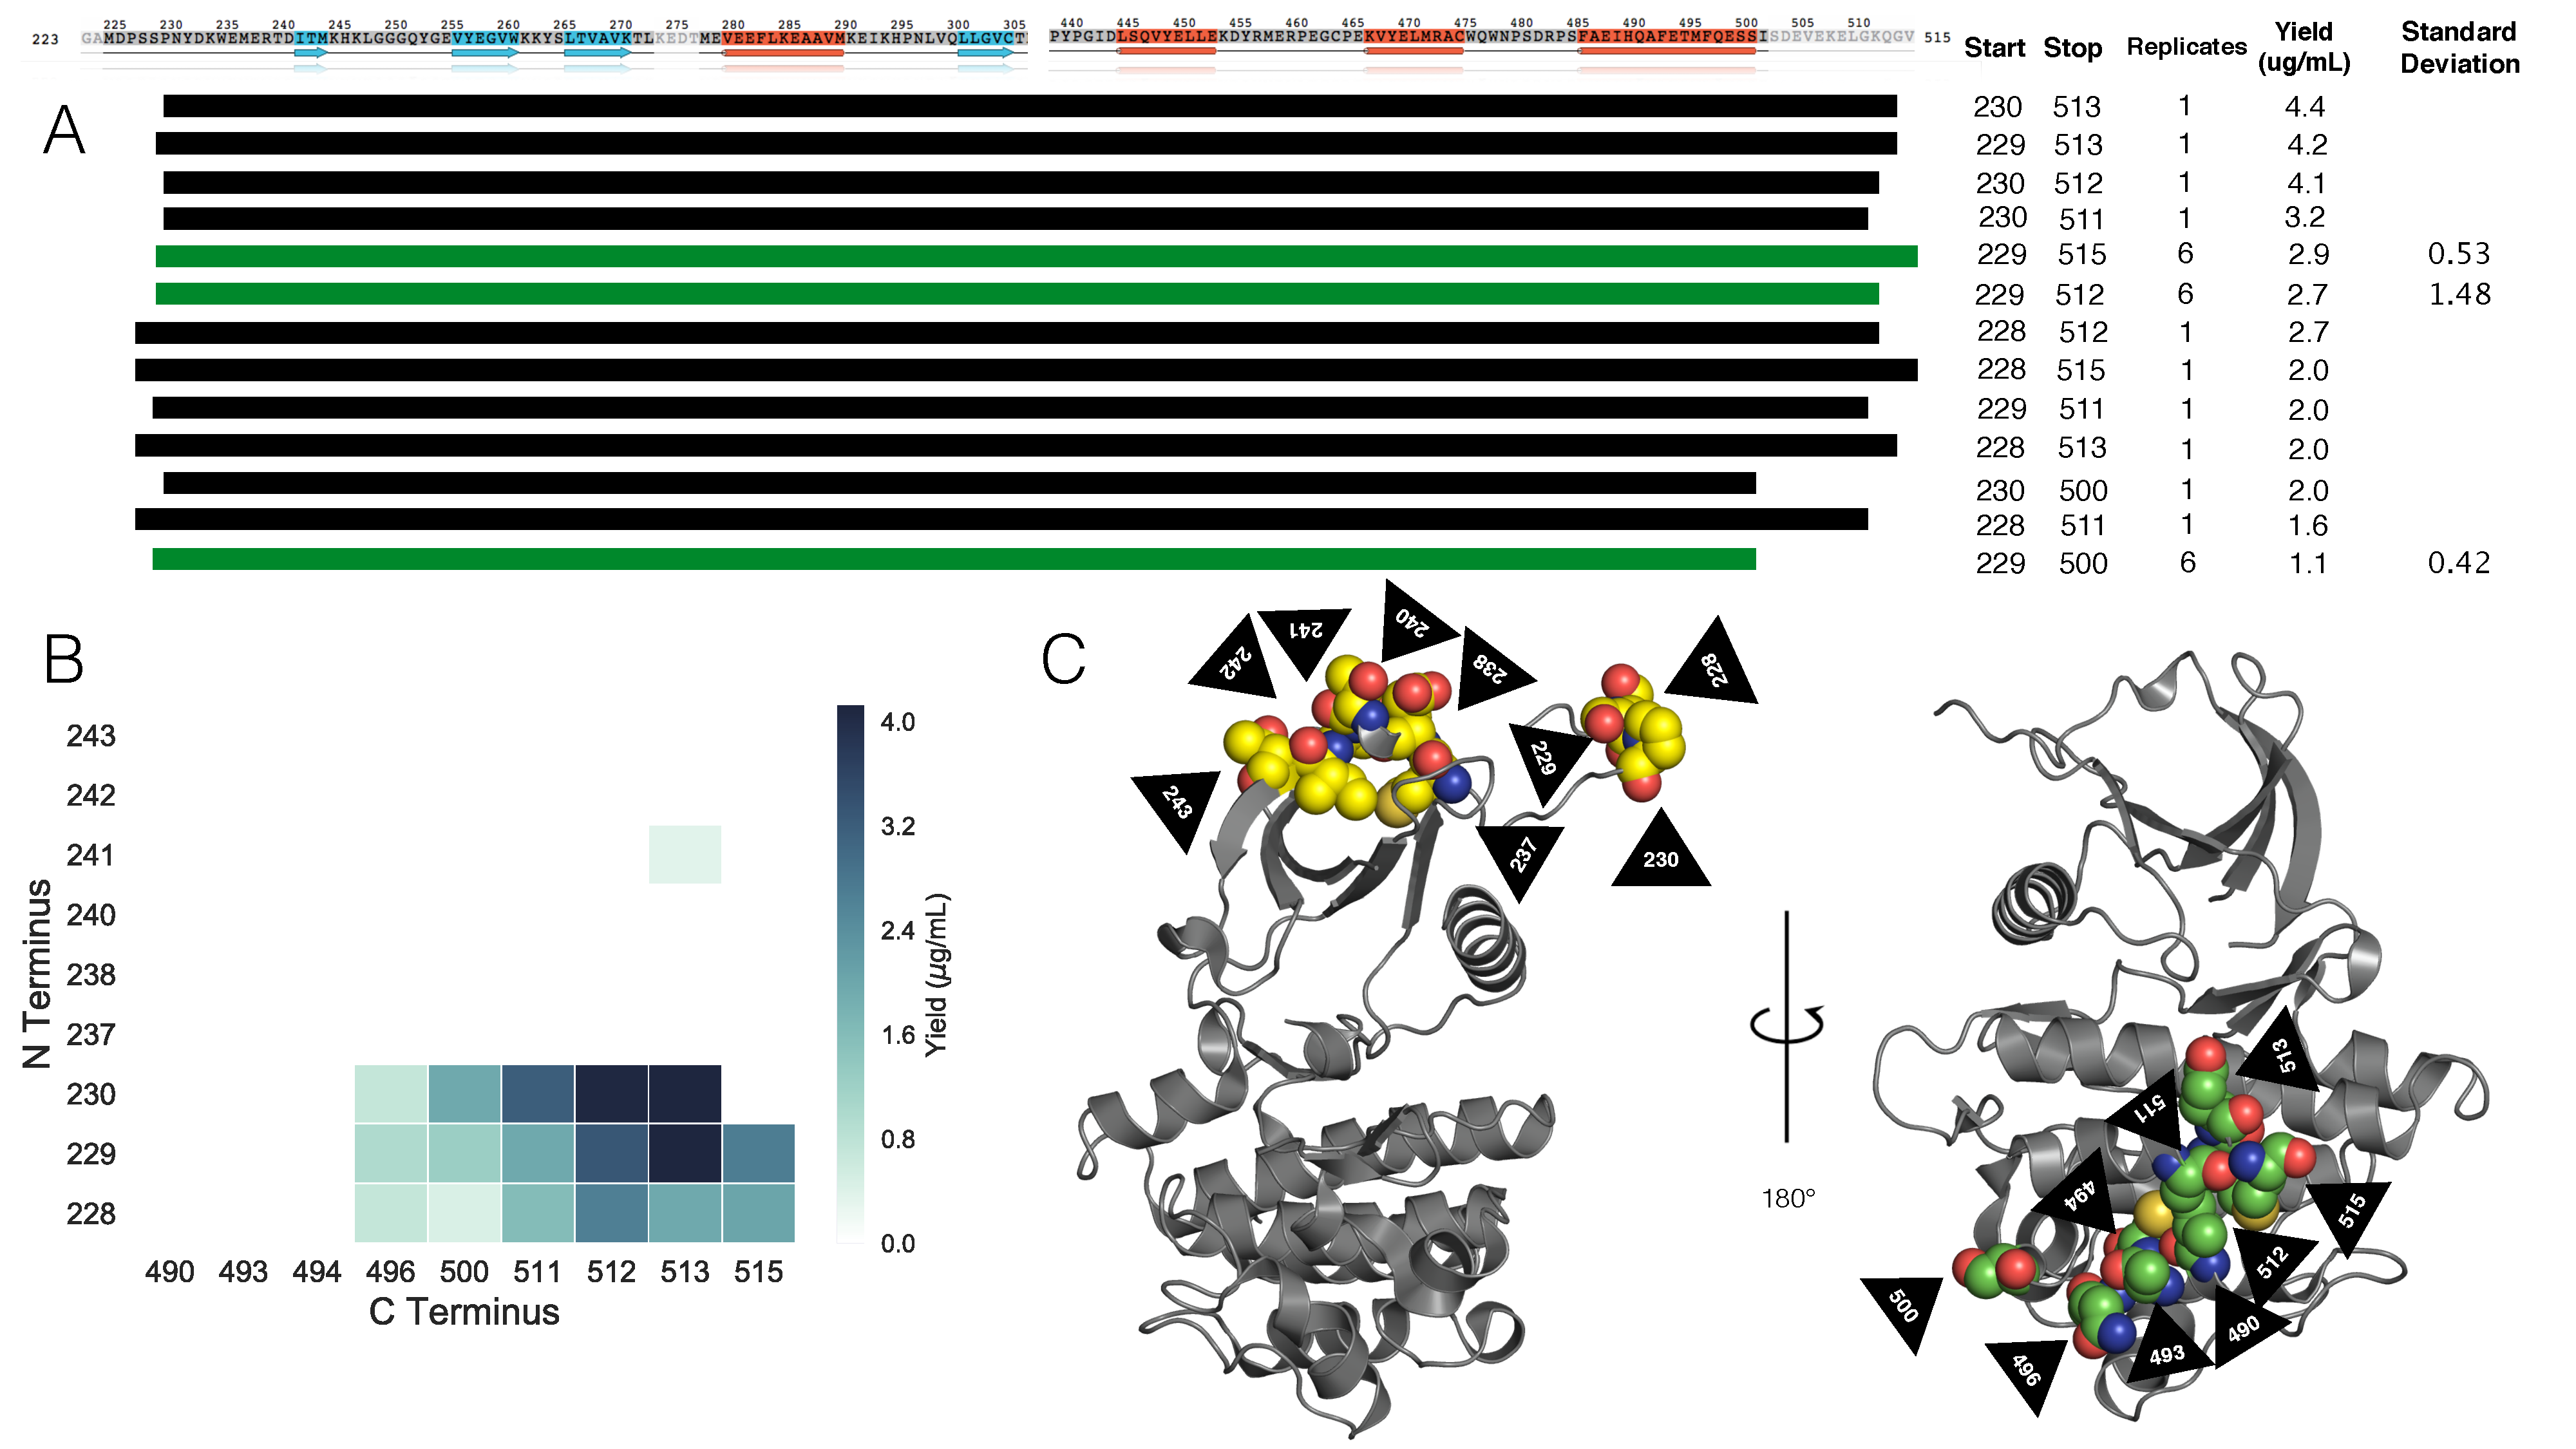
\includegraphics[width=\linewidth]{abl1-construct-wholefigure.pdf}
  \caption{{\bf Abl kinase domain construct expression screen illustrates high sensitivity to construct boundaries.}
  ({\bf A}) Abl kinase domain construct boundaries with highest expression yields. 
  Standard deviations of the yield are listed for control constructs for which six replicates were performed to give an indication of the uncertainty in experimental constructs. Secondary structure is indicated on the sequence. Beta sheets are colored blue and alpha helices are colored orange. 
	({\bf B}) Heatmap showing average yields for constructs with detectable expression as a function of N- and C-terminal construct boundaries.
  ({\bf C}) \emph{left}: PDBID: 2E2B with the nine N-terminal construct boundary amino acids shown as yellow spheres. 
  \emph{right}: PDBID: 4XEY with the nine C-terminal construct boundary amino acids shown as green spheres. 
  Black arrows indicate residue numbers. 
   }
  \label{fig:ab1-const-fig}
\end{fullwidth}
\end{figure}

A detailed explanation of the methods are available in the 'Methods' section, but briefly the impact of construct boundary choice on Abl kinase domain expression was tested as follows. His10-TEV N-terminally tagged wild type Abl constructs\footnote{Parent plasmid is a pET His10 TEV LIC cloning vector and is available on Addgene (Plasmid \#78173).}, which were coexpressed with YopH phosphatase in a 96-well format with control replicates distributed randomly throughout the plate.
His-tagged protein constructs were recovered via a single nickel affinity chromatography step, and construct yields were quantified using microfluidic capillary electrophoresis following thermal denaturation. 
Expression yields are summarized in Figure~\ref{fig:ab1-const-fig}A, and a synthetic gel image from the constructs with detectable expression is shown in Figure~\ref{fig:abl1_caliper_image}. 
Abl construct bands are present at sizes between 29 and 35 kDa (due to the variation in construct boundaries), and YopH phosphatase (which is not His-tagged but has substantial affinity for the nickel beads) is present in all samples at its expected size of 50 kDa. 
Strikingly, despite the fact that N-terminal and C-terminal construct boundaries only varied over 15--25 residues, only a small number of constructs produced detectable expression (Figure~\ref{fig:ab1-const-fig}B). 
As highlighted in Figure~\ref{fig:ab1-const-fig}C (left), the best N-terminal boundaries (residues 228, 229, 230) are located on a disordered strand distant from any secondary structure; N-terminal boundaries closer to the beta sheet of the N-lobe gave poor or no detectable expression (Figure~\ref{fig:ab1-const-fig}B). 
\todo[color=yellow!50]{ Yellow/green sphere depiction of terminal residues in Figure 1C are not helpful. I know it is a lot of effort to adjust these figures, these construct boundaries could be much clearer if only gray ribbon structure is shown with black terminal tags with residue numbers. Spheres and showing side-chains are not essential for this figure.  -MI}
The best C-terminal construct boundaries (residues 511 and 512) occur in an $\alpha$-helix (Figure~\ref{fig:ab1-const-fig}C, right). 
Of note, this $\alpha$-helix is not resolved in PDBID:2E2B~\citep{Horio:2007wo}, suggesting this structural element may only be weakly thermodynamically stable in the absence of additional domains.

Surprisingly, two of the control constructs identified as constructs appearing in crystal structures in the PDB (which differ in construct boundary by only one or two residues) were in the top six expressing constructs (Figure~\ref{fig:ab1-const-fig}A), and were in fact within 60\% of the maximum observed expression yield.
We concluded that transferring construct boundaries from existing kinase domain structural data would be sufficient to at least bias our constructs toward useful expression levels for a large-scale screen of multiple kinases. 

\begin{figure}[t!]
\centering
\begin{fullwidth}
   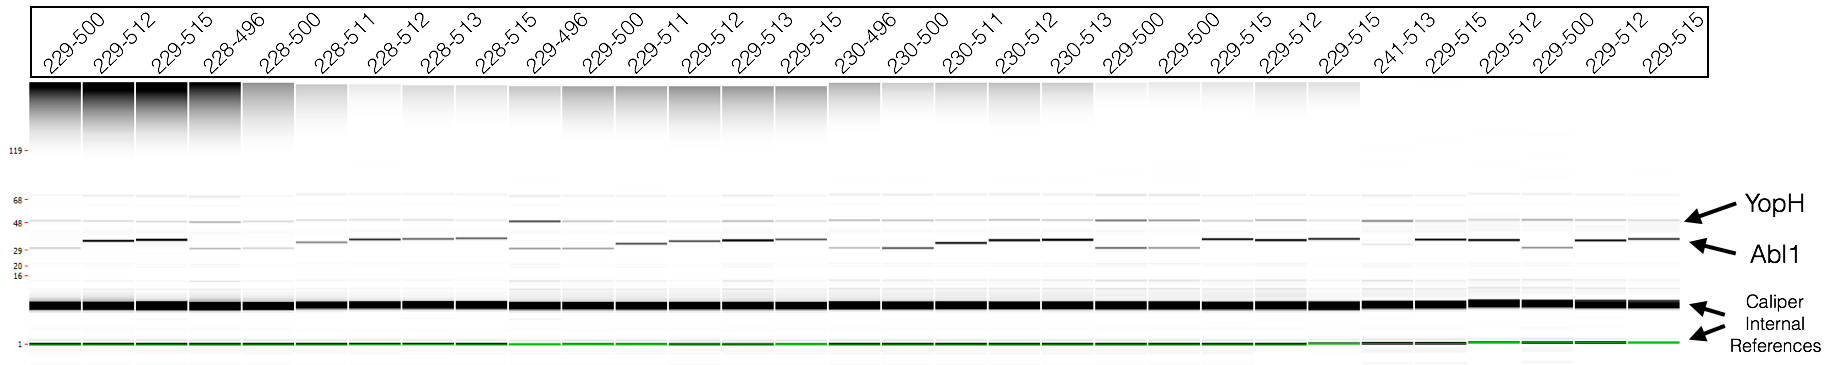
\includegraphics[width=\linewidth]{abl1-construct-gel.png}
  \caption{{\bf Expression yields of Abl kinase domain constructs for all constructs with detectable expression.}
   A synthetic gel image rendering was generated from Caliper GX II microfluidic gel electrophoresis data following nickle affinity purification and thermal denaturation for all Abl constructs with detectable expression. 
   Each well is marked with the Abl kinase domain construct boundaries. 
   Bands for YopH164 phosphatase (50 kDA) and Abl kinsase domain constructs (28--35 kDA) are labeled. 
   }
  \label{fig:abl1_caliper_image}
  \end{fullwidth}
\end{figure}

\subsection{Screen of 96 different kinases finds 52 with useful levels of expression in \emph{E.~coli}}

To begin exploring which human kinase domains can achieve useful expression in \emph{E.~coli} using a simple automatable expression and purification protocol, a panel of kinase domain constructs for 96 kinases, for which bacterial expression has been previously demonstrated (determined from PDB header {\tt EXPRESSION\_SYSTEM} records) were selected using a semi-automated bioinformatics pipeline. 
Briefly, a database was built by querying Uniprot~\citep{uniprot:2017} for human protein kinase domains that were both active and not truncated. 
This query returned a set of target sequences that were then matched to their relevant PDB constructs and filtered for expression system, discarding kinases that did not have any PDB entries with bacterial expression. 
As a final filtering step, the kinases were compared to three purchased kinase plasmid libraries (described in the Methods section), discarding kinases without a match. Construct boundaries were selected from PDB constructs and the SGC plasmid library, both of which have experimental evidence for \emph{E. coli} expression, and subcloned from a plasmid in the purchased library. This process is explained in more detail in the Methods section. 
Selecting the kinases and their constructs for this expression trial in this method rested on the basis of expected success: these specific kinase constructs were bacterially expressed and purified to a degree that a crystal structure could be solved. 
While the expression protocols used to produce protein for crystallographic studies were likely tailored to maximize expression for individual proteins, we considered these kinases to have a high chance of expressing in our semi-automated pipeline where the \emph{same} protocol is utilized for all kinases. 
Statistics of the number of kinases obtained from the PDB mining procedure are shown in Figure~\ref{fig:kinome-expression}A. 
Surprisingly, the most highly sampled family was the CAMK family, suggesting that other researchers may have found this family particularly amenable to bacterial expression.
Based on the results of the previous experiment scanning Abl constructs for expression, we decided to use construct boundaries that were reported in the literature for each kinase. 
This process resulted in a set of 96 plasmid constructs distributed across kinase families (Figure~\ref{fig:kinome-expression}B). 

\begin{figure}[b!]
\centering
  \begin{fullwidth}
   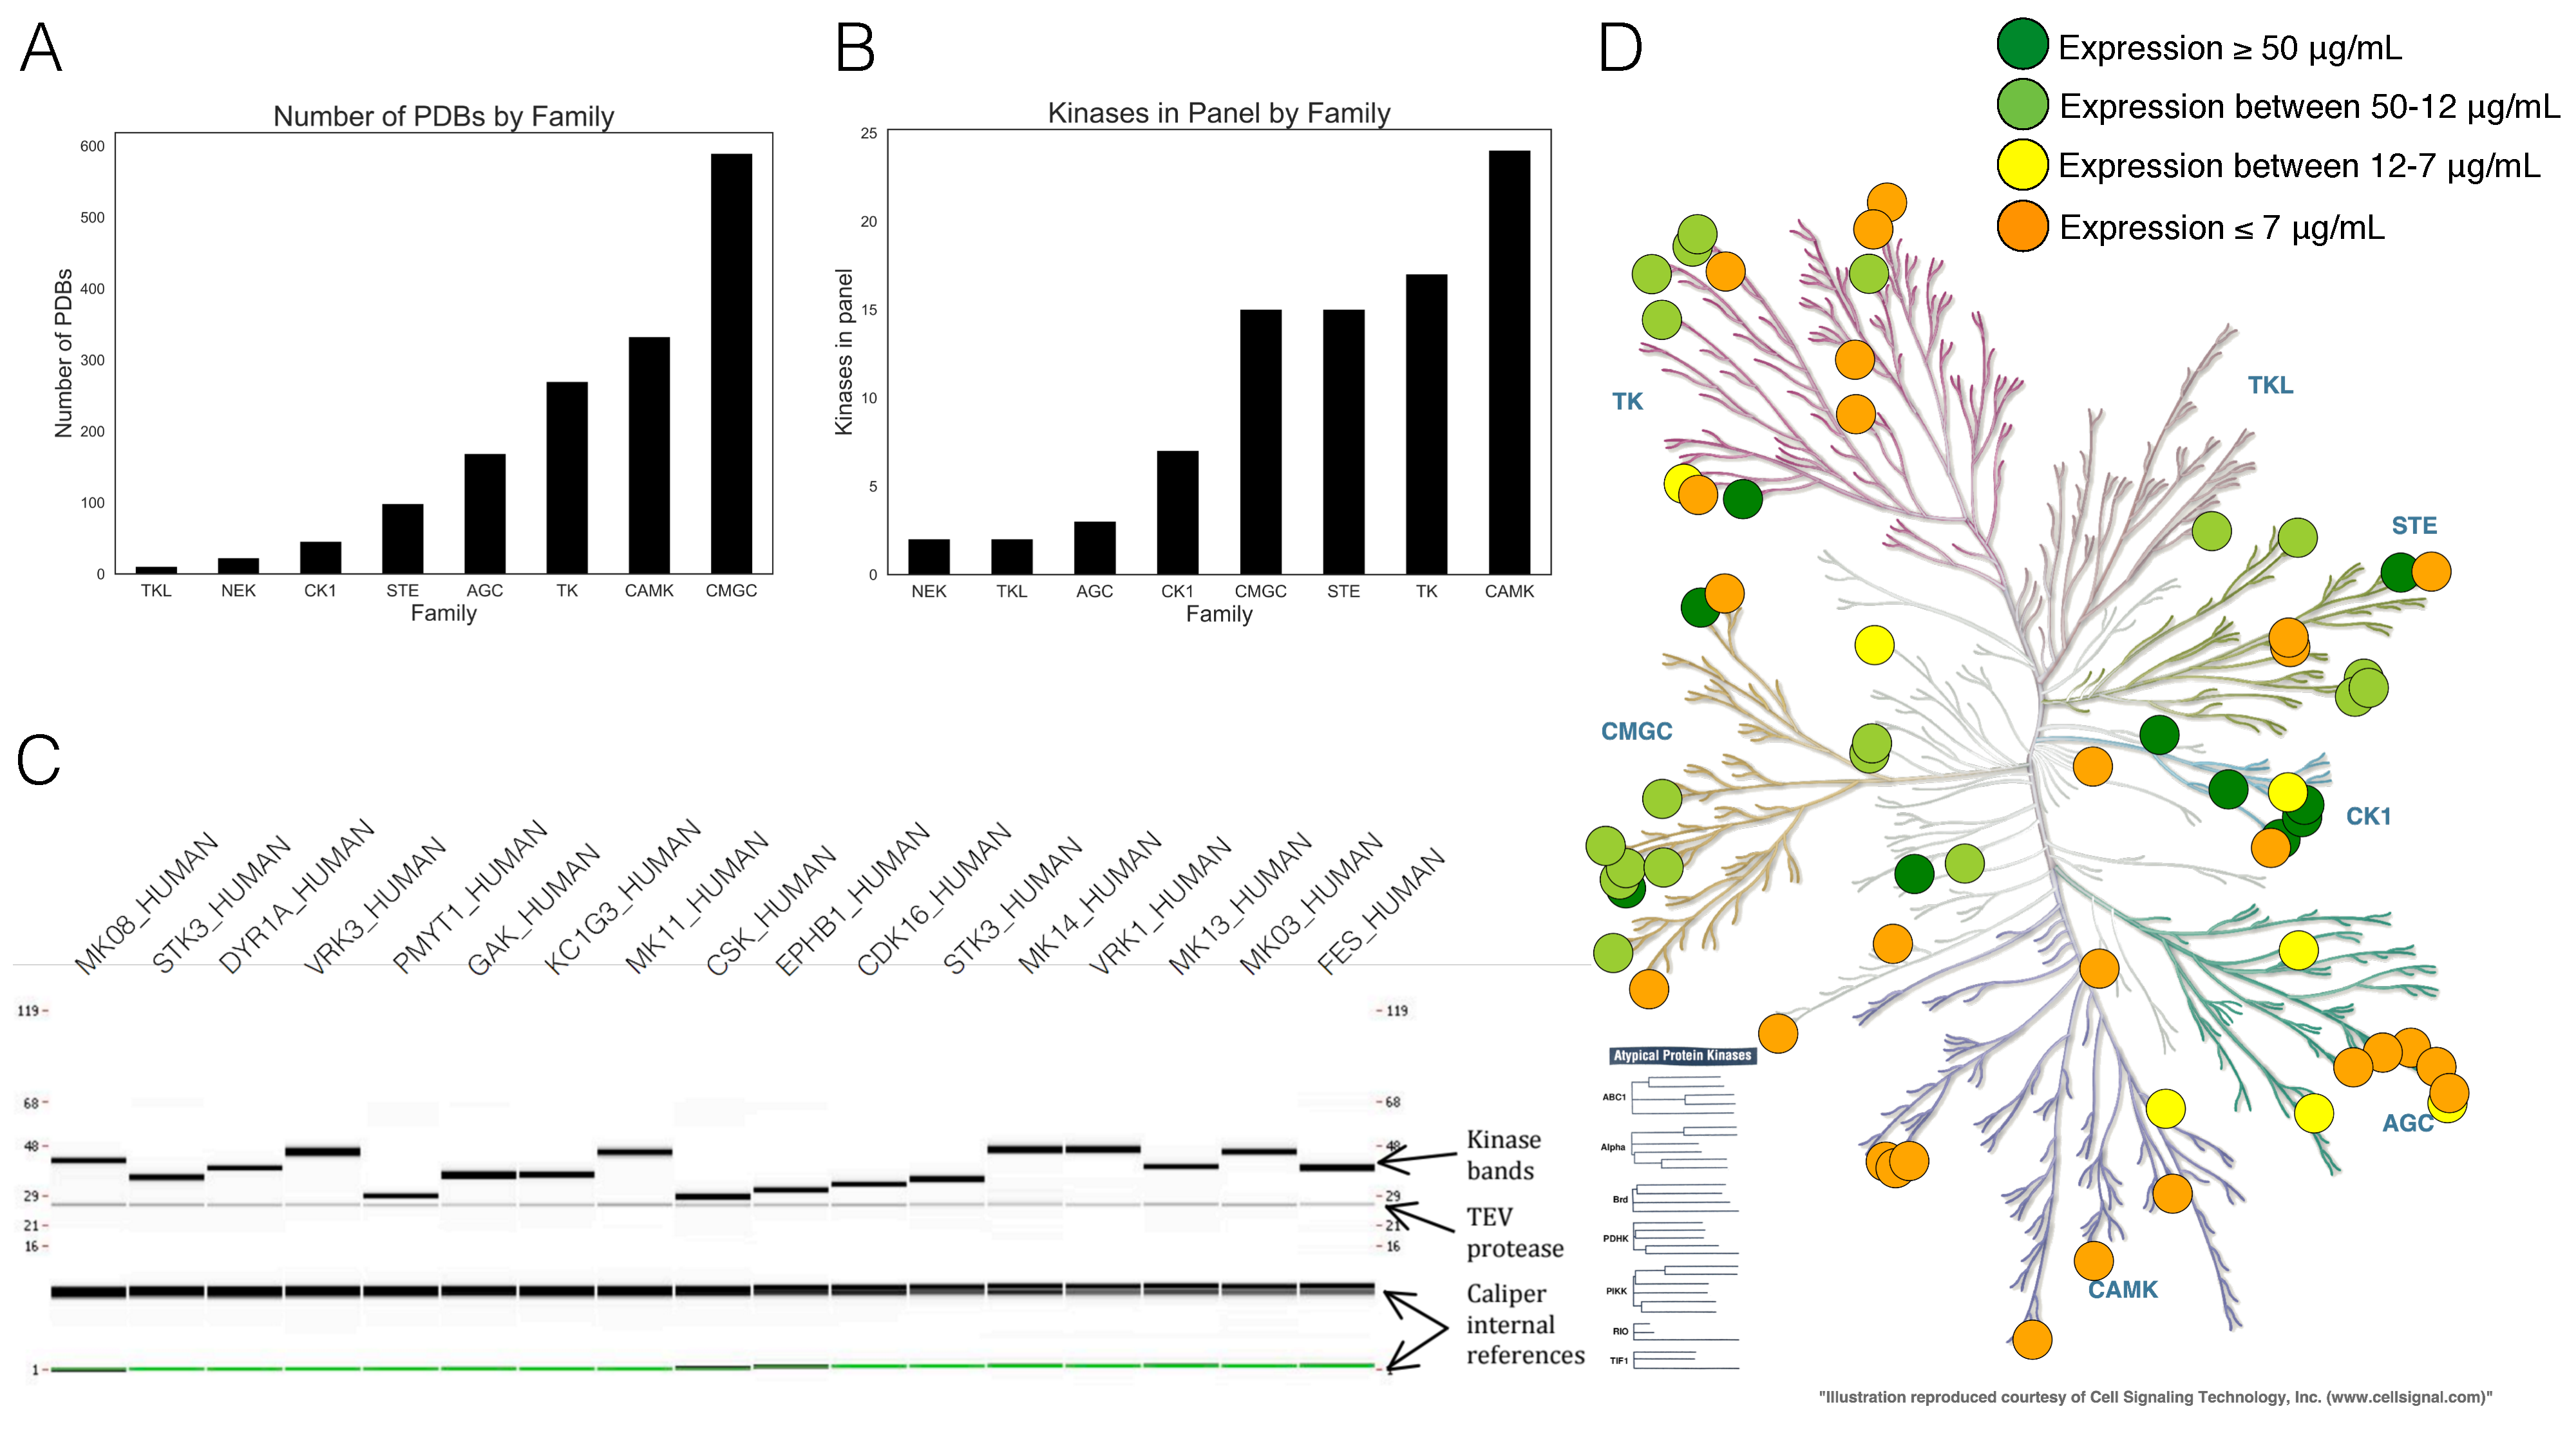
\includegraphics[width=\linewidth]{96-kinase-figure}
  \caption{{\bf Kinome wide search for expressible kinases.}
  ({\bf A}) The number of PDB structures per kinase family, from the database built to select kinases for expression. ({\bf B}) The distribution among familes of candidate kinases in our expression screen. ({\bf C}) Caliper GX II synthetic gel image rendering of the highest expressing kinases, quantified using microfluidic capillary electrophoresis.  ({\bf D}) Kinome distribution of expression based on our 96 kinase screen. Dark green circles represent kinases with expression above 50~$\mu$g/mL culture yield.
  Light green circles represent kinases with expression between 50 and 12~$\mu$g/mL yield.
  Yellow circles represent kinases with expression between 12 and 7~$\mu$g/mL yield.
  Orange circles represent kinases with any expression (even below 2~$\mu$g/mL) up to 7~$\mu$g/mL yield.
  Image made with KinMap: \href{http://www.kinhub.org/kinmap}{http://www.kinhub.org/kinmap}. 
   }
  \label{fig:kinome-expression}
  \end{fullwidth}
\end{figure}

From these, a set of 96 His10-TEV N-terminally tagged kinase domain constructs were generated, coexpressed with phosphatase \emph{E.~coli}, purified via nickel bead pulldown, and quantified via microfluidic gel electrophoresis.
The 96 kinases were coexpressed with either Lambda phosphatase (for Ser/Thr kinases) or a truncated form of YopH phosphatase\footnote{Yoph164 phosphatase, engineered to minimize intrinsic affinity for nickel purification resin by the QB3 MacroLab based on parent plasmid pCDFDuet1-YOPH, a gift from the Kuriyan Lab.} (for Tyr kinases). 

Instead of eluting with imidazole, purified kinase was cleaved off nickel beads by the addition of 10\% TEV protease to minimize phosphatase contamination in the resulting eluate in order to assess whether resulting yields would be sufficient (and sufficiently free of phosphatase) to permit activity assays.
While the initial panel of 96 kinases was well distributed amongst the kinase families (Figure~\ref{fig:kinome-expression}B), the most highly expressing kinases (yield of more than 12~$\mu$g/mL kinase) were not evenly distributed (Figure~\ref{fig:kinome-expression}D). 
52 kinases demonstrated a useful level of soluble protein expression, here defined as greater than 2 $\mu$g/mL, na\"{i}vely expected to scale up to better than 2 mg/L culture (Table~\ref{expression_table}). 
Some kinases (shaded green in (Table~\ref{expression_table}) demonstrated very high levels of expression, while others (shaded orange in (Table~\ref{expression_table}) would likely benefit from further rounds of construct boundary optimization or solubility tags to boost soluble expression. 
The 17 most highly expressing kinases showed relatively high purity after elution, though we note that eluting via TEV site cleavage results in a quantity of TEV protease in the eluate (Figure~\ref{fig:kinome-expression}C), but does not cause the elution of the His-tagged phosphatases. 

Constructs with expression yields above 2 $\mu$g/mL have been made available via {\bf Addgene}:\\
\url{https://www.addgene.org/kits/chodera-kinase-domains}
\begin{table}[h!]
\centering
\caption{{\bf Kinase domain constructs with yields >2 $\mu$g/mL culture for 96-kinase expression screen.} 
Kinases are listed by Uniprot designation and whether they were co-expressed with Lambda or truncated YopH164 phosphatase.
Yield (determined by Caliper GX II quantitation of the expected size band) reported in $\mu$g/mL culture, where total eluate volume was 120 $\mu$L from 900 $\mu$L bacterial culture. 
Yields are shaded green (yield > 12 $\mu$g/mL), yellow (12 > yield > 7 $\mu$g/mL) and orange (yield <7 $\mu$g/mL); kinase domain constructs with yields that were undetectable or < 2 $\mu$g/mL are not listed.  
$\ddag$ denotes that the second kinase domain of KS6A1\_HUMAN was expressed; all other kinases were the first or only kinase domain occurring in the ORF.
Construct boundaries are listed in UniProt residue numbering for the UniProt canonical isoform.
A sortable table of expression yields and corresponding constructs is available at \url{http://choderalab.org/kinome-expression}
}
\label{expression_table}
\scriptsize
\begin{tabular}{p{3cm}cp{3.5cm}p{3cm}c}
\toprule
\bf{kinase} & \bf{construct} & \bf{Plasmid Source and ID}&\bf{phosphatase} & \bf{yield ($\mu$g/mL)} \\
\midrule
MK14\_HUMAN & 1--360& Addgene 23865&	Lambda                    & \cellcolor{forestgreen!55}\bf{70.7}                            \\
VRK3\_HUMAN & 24--352&SGC Oxford	VRK3A-c016 & Lambda                    & \cellcolor{forestgreen!55}\bf{67.5}                            \\
GAK\_HUMAN  & 24--359& SGC Oxford GAKA-c006 & Lambda                    & \cellcolor{forestgreen!55}\bf{64.7}                            \\
CSK\_HUMAN  & 186--450& Addgene	23941 & YopH         & \cellcolor{forestgreen!55}\bf{62.5}                            \\
VRK1\_HUMAN & 3--364& Addgene	23496 & Lambda                    & \cellcolor{forestgreen!55}\bf{62.3}                            \\
KC1G3\_HUMAN & 24--351 & SGC Oxford CSNK1G3A-c002 & Lambda                    & \cellcolor{forestgreen!55}\bf{56.3}                            \\
FES\_HUMAN  & 448--822 & Addgene 23876 & YopH         & \cellcolor{forestgreen!55}\bf{44.0}                            \\
PMYT1\_HUMAN & 24--311& SGC Oxford	PKMYT1A-c004 & Lambda                    & \cellcolor{forestgreen!55}\bf{38.0}                            \\
MK03\_HUMAN  & 1--379 & Addgene	23509 &Lambda                    & \cellcolor{forestgreen!55}\bf{36.4}                            \\
STK3\_HUMAN  &16--313 & Addgene	23818 & Lambda                    & \cellcolor{forestgreen!55}\bf{34.3}                            \\
DYR1A\_HUMAN & 24--382& SGC Oxford	DYRK1AA-c004 & Lambda                    & \cellcolor{forestgreen!55}\bf{34.1}                            \\
KC1G1\_HUMAN & 24--331& SGC Oxford	CSNK1G1A-c013 & Lambda                    & \cellcolor{forestgreen!55}\bf{34.1}                            \\
MK11\_HUMAN  & 24--369 & SGC Oxford	MAPK11A-c007 & Lambda                    & \cellcolor{forestgreen!55}\bf{31.7}                            \\
MK13\_HUMAN  &1--352 & Addgene 23739&Lambda                    & \cellcolor{forestgreen!55}\bf{31.7}                            \\
EPHB1\_HUMAN & 602--896& Addgene 23930& YopH         & \cellcolor{forestgreen!55}\bf{28.9}                            \\
MK08\_HUMAN  & 1--363 & HIP pJP1520 HsCD00038084 & Lambda                    & \cellcolor{forestgreen!55}\bf{28.5}                            \\
CDK16\_HUMAN &163--478 & Addgene 23754 & Lambda                    & \cellcolor{forestgreen!55}\bf{26.9}                            \\
EPHB2\_HUMAN &604--898& HIP pJP1520 HsCD00038588 & YopH         & \cellcolor{forestgreen!55}\bf{25.1}                            \\
PAK4\_HUMAN  &291--591 & addgene 23713 & Lambda                    & \cellcolor{forestgreen!55}\bf{23.9}                            \\
CDKL1\_HUMAN & 2--304& SGC Oxford CDKL1A-c024 & Lambda                    & \cellcolor{forestgreen!55}\bf{23.2}                            \\
SRC\_HUMAN   & 254--536 & Addgene 23934 & YopH         & \cellcolor{forestgreen!55}\bf{22.0}                            \\
STK16\_HUMAN & 24--316 & SGC Oxford STK16A-c002 & Lambda                    & \cellcolor{forestgreen!55}\bf{20.7}                            \\
MAPK3\_HUMAN & 33--349 & Addgene 23790 & Lambda                    & \cellcolor{forestgreen!55}\bf{18.8}                            \\
PAK6\_HUMAN  & 383--681 & Addgene 23833 & Lambda                    & \cellcolor{forestgreen!55}\bf{18.0}                            \\
CSK22\_HUMAN & 1--334 & HIP pJP1520 HsCD00037966 & Lambda                    & \cellcolor{forestgreen!55}\bf{17.9}                            \\
MERTK\_HUMAN & 570--864 & Addgene 23900 & YopH         & \cellcolor{forestgreen!55}\bf{16.8}                            \\
PAK7\_HUMAN  & 24--318 & SGC Oxford PAK5A-c011 & Lambda                    & \cellcolor{forestgreen!55}\bf{14.7}                            \\
CSK21\_HUMAN & 1--335 & Addgene 23678 & Lambda                    & \cellcolor{forestgreen!55}\bf{14.5}                            \\
EPHA3\_HUMAN & 606--947 & Addgene 23911 & YopH         & \cellcolor{forestgreen!55}\bf{14.1}                            \\
BMPR2\_HUMAN & 1--329 & SGC Oxford BMPR2A-c019 & Lambda                    & \cellcolor{forestgreen!55}\bf{14.1}                            \\
M3K5\_HUMAN  & 659--951 & HIP pJP1520 HsCD00038752 & Lambda                    & \cellcolor{forestgreen!55}\bf{14.0}                            \\
KCC2G\_HUMAN & 24--334 & SGC Oxford CAMK2GA-c006 & Lambda                    & \cellcolor{forestgreen!55}\bf{13.3}                            \\
E2AK2\_HUMAN & 254--551 & HIP pJP1520 HsCD00038350 & Lambda                    & \cellcolor{yellow!55}\bf{11.6}                            \\
MK01\_HUMAN  & 1--360 & HIP pJP1520 HsCD00038281 & Lambda                    & \cellcolor{yellow!55}\bf{11.2}                            \\
CSKP\_HUMAN  & 1--340 & HIP pJP1520 HsCD00038384 & Lambda                    & \cellcolor{yellow!55}\bf{10.1}                            \\
CHK2\_HUMAN  & 210--531 & Addgene 23843 & Lambda                    & \cellcolor{yellow!55}\bf{8.1}                             \\
KC1G2\_HUMAN & 4--312 & SGC Oxford CSNK1G2A-c002 & Lambda                    & \cellcolor{yellow!55}\bf{7.6}                             \\
DMPK\_HUMAN  &2 4--433 & SGC Oxford DMPK1A-c026 & Lambda                    & \cellcolor{yellow!55}\bf{7.6}                             \\
KCC2B\_HUMAN & 11--303 & Addgene 23820 & Lambda                    & \cellcolor{yellow!55}\bf{7.1}                             \\
FGFR1\_HUMAN & 456--763 & Addgene 23922 & YopH         & \cellcolor{orange!55}\bf{6.1}                             \\
KS6A1\_HUMAN$^\ddag$ &413--735 & SGC Oxford RPS6KA1A-c036 &   Lambda                    & \cellcolor{orange!55}\bf{5.7}                             \\
DAPK3\_HUMAN & 9--289 & Addgene 23436 &  Lambda                    & \cellcolor{orange!55}\bf{4.0}                             \\
STK10\_HUMAN & 18--317 & HIP pJP1520 HsCD00038077 &  Lambda                    & \cellcolor{orange!55}\bf{3.7}                             \\
KC1D\_HUMAN  & 1--294 & Addgene 23796 & Lambda                    & \cellcolor{orange!55}\bf{3.7}                             \\
KC1E\_HUMAN  & 1--294 & Addgene 23797 & Lambda                    & \cellcolor{orange!55}\bf{3.5}                             \\
NEK1\_HUMAN  & 23--350 & SGC Oxford NEK1A-c011 & Lambda                    & \cellcolor{orange!55}\bf{3.3}                             \\
CDK2\_HUMAN  & 1--297 & Addgene 23777 & Lambda                    & \cellcolor{orange!55}\bf{3.1}                             \\
ABL1\_HUMAN  & 229--512 & HIP pJP1520 HsCD00038619 & YopH         & \cellcolor{orange!55}\bf{2.5}                             \\
DAPK1\_HUMAN & 2--285 & HIP pJP1520 HsCD00038376 & Lambda                    & \cellcolor{orange!55}\bf{2.4}                             \\
DYRK2\_HUMAN & 23--417 & SGC Oxford DYRK2A-c023 & Lambda                    & \cellcolor{orange!55}\bf{2.4}                             \\
HASP\_HUMAN  & 24--357 & SGC Oxford GSG2A-c009 &  Lambda                    & \cellcolor{orange!55}\bf{2.3}                             \\
FGFR3\_HUMAN & 449--759	& Addgene 23933 & YopH         & \cellcolor{orange!55}\bf{2.3}                             \\
\bottomrule
\end{tabular}
\end{table}

\subsection{Expressing clinically-derived Src and Abl mutants}

The advent of next-generation sequencing technology has enabled generation of massive datasets rich with missense alterations in kinases observed directly in the clinic~\citep{Varghese:2014jw,Zehir:2017ib,Garraway:2013kn}, and has been particularly transformative in the field of oncology. 
To determine how well our kinase domain constructs and automated expression/purification protocol support the expression of clinically-identified kinase domain missense mutants for biophysical, biochemical, and structural characterization, we attempted to express 96 missense mutations mined from sequencing studies of cancer patients, both from publicly available sources as well a private clinical tumor sequencing dataset from Memorial Sloan Kettering~\citep{Zehir:2017ib} sequenced as part of the MSK-IMPACT panel~\citep{msk-impact}, as identified via the MSK cBioPortal~\citep{cBioPortal}. 

Similar to the expression screen above, a database was built focusing on the kinases we found to be expressible in \emph{E.~coli}. 
To add the mutation data, we retrieved public datasets from cBioPortal~\citep{Cerami:2012eu,Gao:2013kd} along with annotations from Oncotator~\citep{Ramos:2015ew} through their respective web service APIs.
We then added mutations and annotations from the private dataset at MSKCC by extracting the mutations from a local copy of the dataset and retrieving annotations from Oncotator. 
The annotated mutations were filtered for mutations that occurred within the construct boundaries of the kinase domains for our expressible kinases. 
We found 63 clinical mutations appearing within our kinase domain construct boundaries in Abl and 61 in Src. 
We subsequently selected 48 mutants for Abl and 46 for Src to express, aiming for a panel of mutants that were distributed throughout the entire kinase domain (Figure~\ref{fig:96-mutant-fig}A). Wild type Src and Abl were included as controls. 
The mutants were engineered into the Src and Abl plasmids from the 96 kinase expression screen using mutagenesis, and coexpressed in \emph{E.~coli} with YopH164 phosphatase. 
Mutants with expression yields above 2$\mu$g/mL are shown in Table~\ref{mut-expression_table}, while all of the mutants are shown in Figure~\ref{fig:96-mutant-fig}A. 
A synthetic gel image produced from microfluidic gel electrophoresis of thermally denatured protein eluate for all of the mutants is shown in Figure~\ref{fig:96-mutant-fig}B.
\todo[color=yellow!50]{ In synthetic gel images of Fig.4B we should label kinase domains, TEV and phosphotase bands. Internal reference bands of Caliper are especially confusing if they are not labelled. -MI}
While the vast majority of the Src mutants expressed at a usable level, many of the Abl mutants expressed below the 2$\mu$g/mL threshold. 
This can primarily be attributed to the low level of expression for wild-type Abl construct (Table~\ref{expression_table}). 
In instances where kinase activity is not required, this yield could be increased using inactivating mutations~\citep{seeliger:2005:protein-sci:kinase-expression}. 


\begin{figure}[h!]
\centering
\begin{fullwidth}
   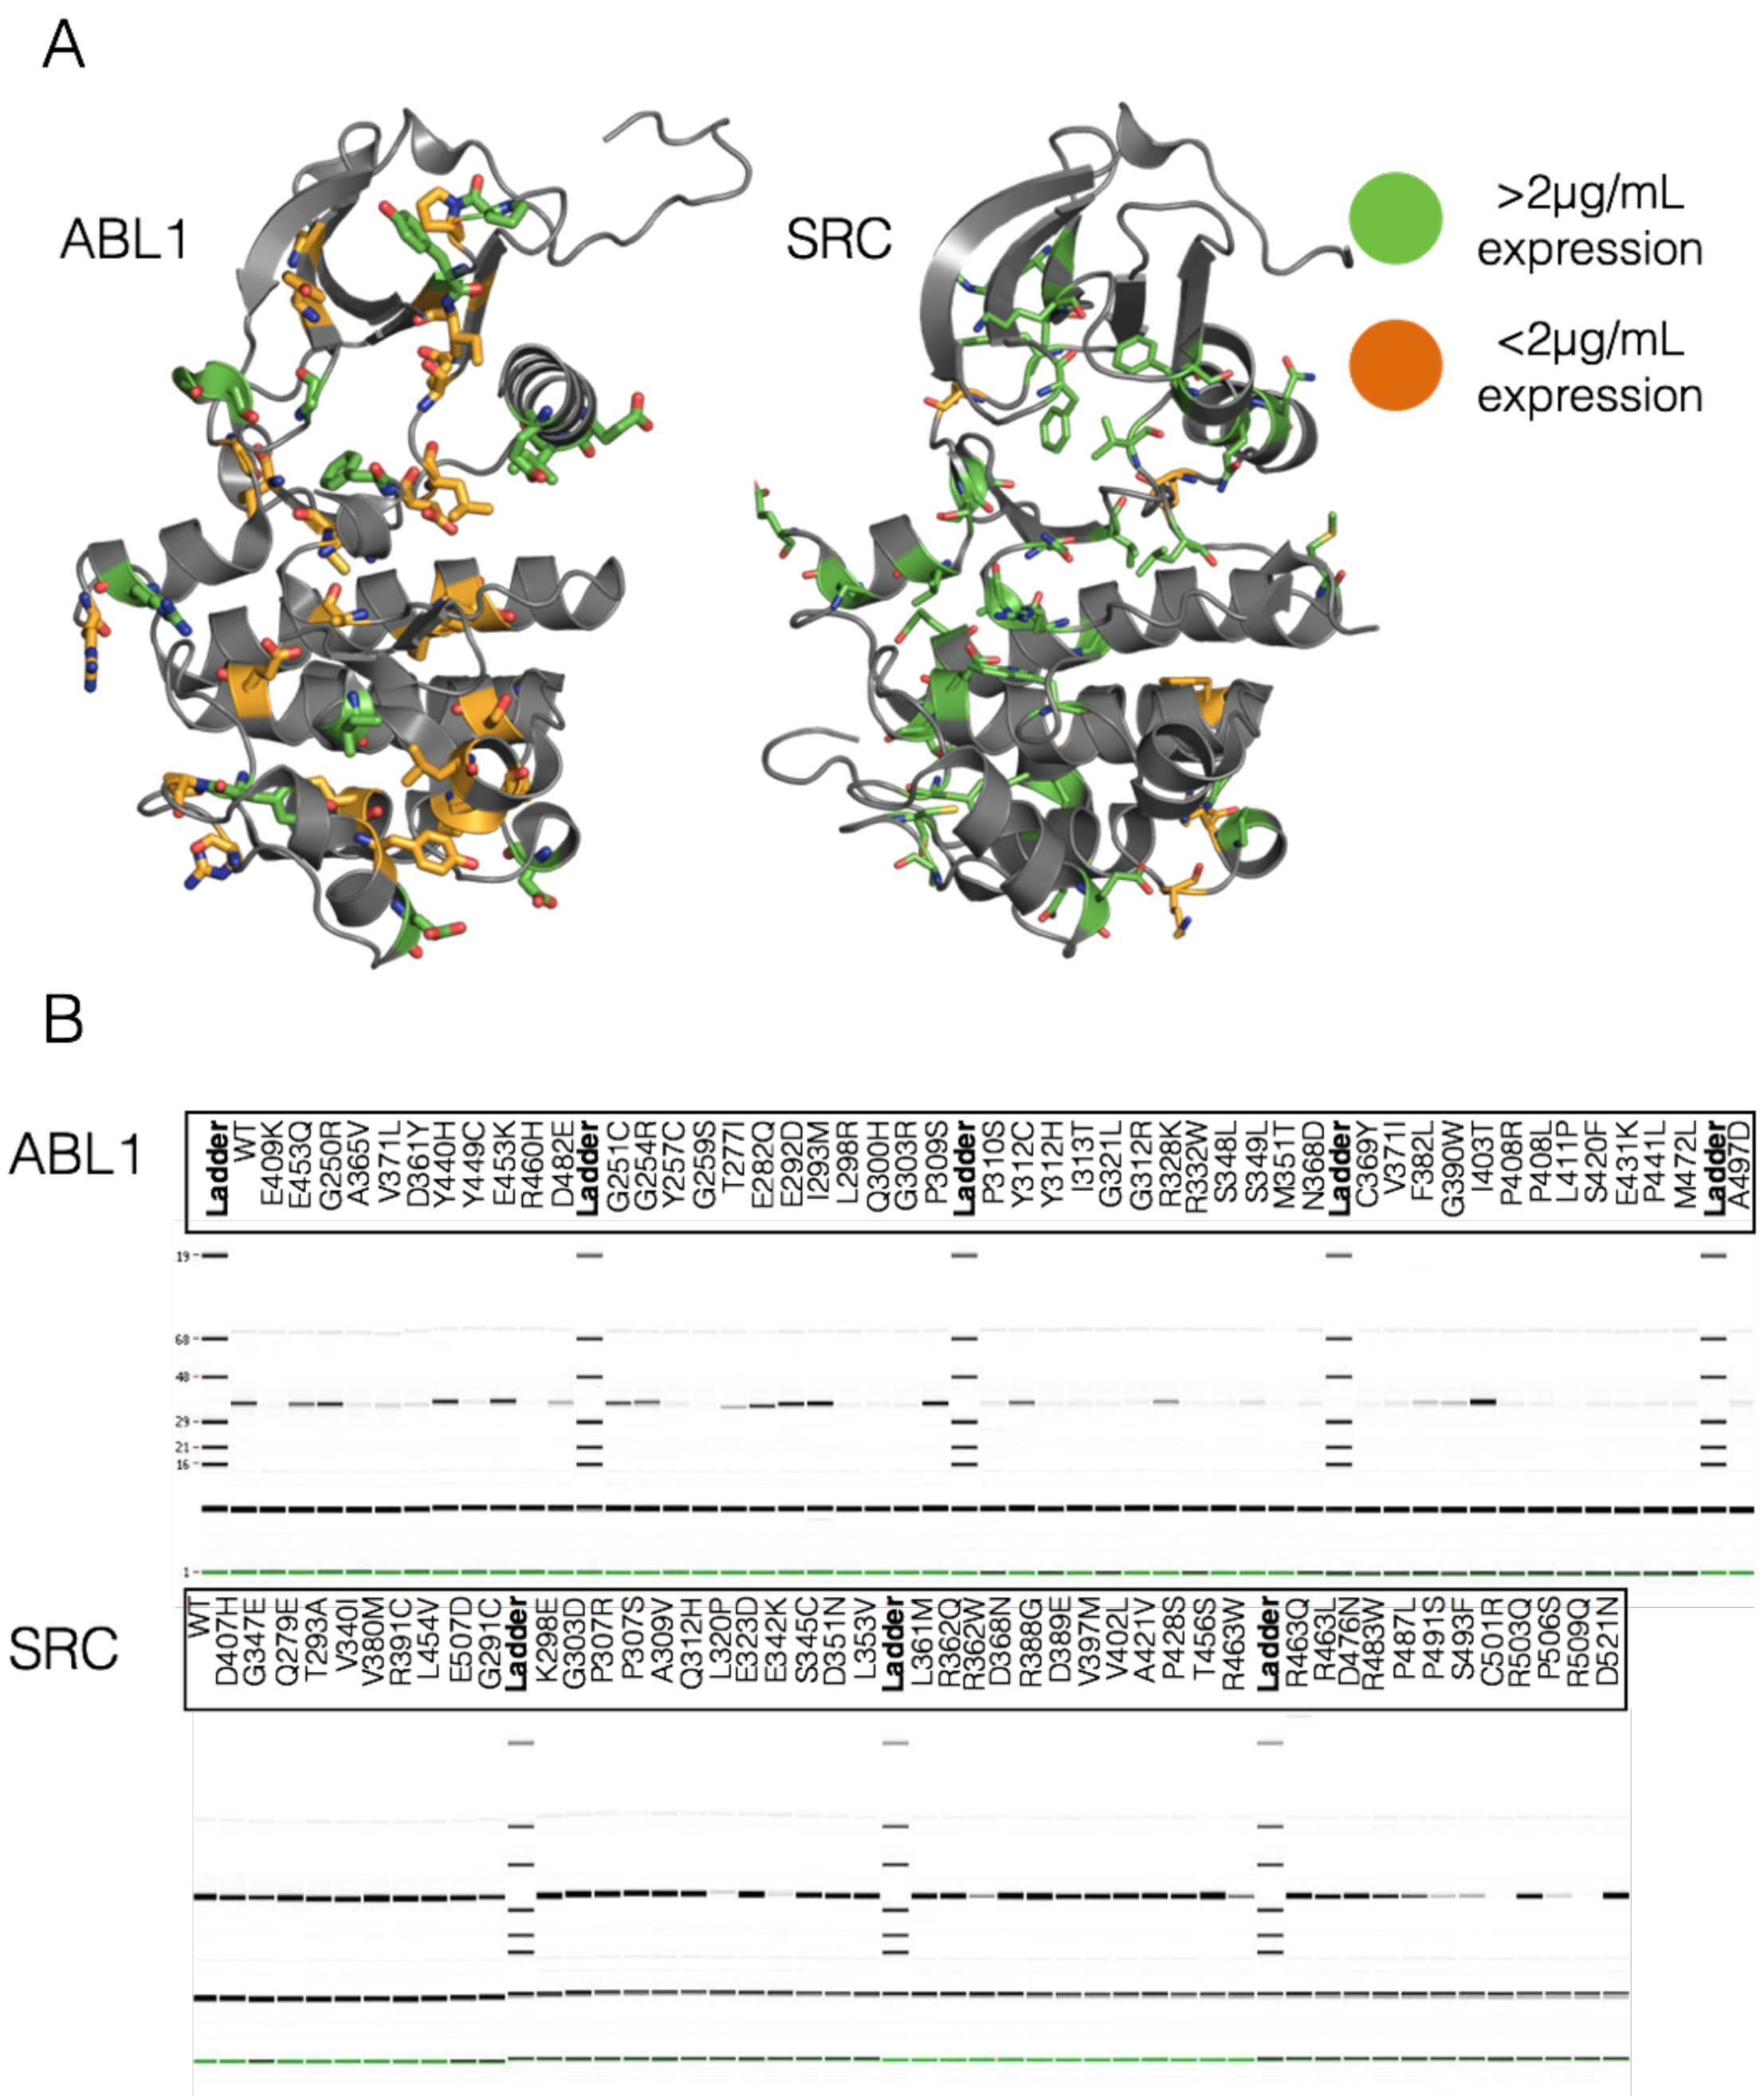
\includegraphics[width=0.9\linewidth]{96-mutant-finalfigure.pdf}
   
  \caption{{\bf Expression yields for engineered clinically-derived Src and Abl missense mutants.}
  ({\bf A}) All Abl and Src clinically-identified mutants assessed in the expression screen are displayed as sticks. 
  Mutants with expression yields >2$\mu$g/mL are colored green, while those with yields <2$\mu$g/mL are colored orange. 
  Rendered structures are PDBID:2E2B (Abl) and PDBID:4MXO (Src)~\citep{Levinson:2014gi}.
  ({\bf B}) Synthetic gel images showing ABl (\emph{top}) or Src (\emph{bottom}) expression, with wells labeled by missense mutation.  Yield  was determined by Caliper GX II quantitation of the expected size band and reported in $\mu$g/mL culture, where total eluate volume was 120 $\mu$L following nickel bead pulldown purification from 900 $\mu$L bacterial culture.
   }
  \label{fig:96-mutant-fig}
\end{fullwidth}
\end{figure}

\begin{table}[h!]
\centering
\caption{{\bf Expression yields for engineered clinical missense mutants of Src and Abl kinase domains with yields > 2 $\mu$g/mL culture.} 
Src and Abl kinase domain constructs with engineered clinical mutations with expression yields > 2$\mu$g/mL culture are listed, sorted by yield. 
Yield  was determined by Caliper GX II quantitation of the expected size band and reported in $\mu$g/mL culture, where total eluate volume was 80 $\mu$L purified from 900 $\mu$L bacterial culture.
Wild-type (WT) controls for both Src and Abl (here, a single well for each) are shown as the first entry for each gene. 
}
\label{mut-expression_table}
\scriptsize
\begin{threeparttable}
\begin{tabular}{ccccc}
\toprule
\bf{Abl1 (229--512)} & \bf{Mutation}\tnote{1} & \bf{Functional Impact Score}\tnote{2} & \bf{yield ($\mu$g/mL)} & \bf{\% of WT expression} \\ 
\midrule
 & WT & --& 5.1 & -- \\
 & I403T & Low & 17.8 & 350 \\
& I293M & Low &9.8 & 193 \\
 & P309S & Neutral & 7.8 & 153 \\
 & E453K & Low & 7.3 & 144 \\
 & Y440H & Medium & 7.1 & 140 \\
 & E292D & Low & 6.9 & 135 \\
 & G251C & High & 5.2 & 102 \\
 & E282Q & Neutral & 5.1 & 102 \\
 & G250R & Neutral & 5.1 & 100 \\
& G254R & High & 5.0 & 98 \\
 & Y312C & Neutral & 4.7 & 93 \\
& E453Q & Low & 3.7 & 73 \\
& R328K & Low & 3.5 & 69 \\
 & D482E & Neutral & 2.5 & 49 \\
 & F382L & Medium & 2.1 & 41 \\
 & G390W & Medium & 2.1 & 41 \\
\toprule
\bf{Src (254--536) }& \bf{Mutation}\tnote{1} & \bf{Functional Impact Score}\tnote{2} & \bf{yield ($\mu$g/mL)} & \bf{\% of WT expression} \\ 
\midrule
& WT& -- & 35.7 & -- \\
& T456S & Neutral& 80.9 & 227 \\
 &R388G & Medium & 61.5 & 172 \\
 &K298E & High & 54.5 & 153 \\
 &V380M & Neutral & 51.7 & 145 \\
 &D368N & Neutral & 49.9 & 140 \\
 &D521N & Low & 42.8 & 120 \\
 &R463Q & Neutral & 38.4 & 108 \\
 &R391C & Neutral & 37.5 & 105 \\
 &E323D & Low & 37.2 & 104 \\
 &A309V & Low & 35.q & 98 \\
 &G303D & Neutral & 34.1 & 96 \\
 &R362Q & Neutral & 33.6 & 94 \\
 &L361M & Medium & 31.7 & 89 \\
 &A421V & Neutral & 30.7 & 86 \\
 &V402L & Neutral & 30.6 & 86 \\
 &V397M & Medium & 29.8 & 84 \\
 &Q278E & Neutral & 29.6 & 83 \\
 &Q312H & Low & 29.5& 83 \\
 &L353V & Medium & 29.0 & 81 \\
 &L454V & Neutral & 29.0 & 81 \\
 &P307R & Neutral & 28.6 & 80 \\
 &V340I & Low & 28.0 & 78 \\
 &P307S & Neutral & 24.2 & 68 \\
 &D476N & Neutral & 23.3 & 65 \\
 &D351N & Neutral & 22.9 & 64 \\
 &T293A & Neutral &  22.2 & 62 \\
 &S345C & Low & 22.2 & 62 \\
 &P428S & Medium & 22.2 & 62 \\
 &E507D & Neutral & 20.7 & 58 \\
 &D389E & High & 20.0 & 56 \\
 &R503Q & Neutral & 17.3 & 49 \\
 &D407H & High & 15.9 & 45 \\
 &R463L & Neutral & 14.9 & 42 \\
 &G291C & Medium & 11.9 & 33 \\
 &G347E & Medium & 10.2 & 29 \\
 &R483W & High & 9.8 & 27 \\
 &P487L & Medium & 6.0 & 17 \\
 &R463W & Medium & 5.2 & 15 \\
 &R362W & Low & 3.9 & 11 \\
 &S493F & Low &  3.0 & 8 \\
 &P491S & Low &  2.2 & 6 \\
\bottomrule
\end{tabular}
\begin{tablenotes}
\item[1] Using Uniprot amino acid sequence numbering
\item[2] MutationAssesor Score~\citep{reva_determinants_2007,doi:10.1093/nar/gkr407}, predicts the impact of missense mutations by looking at how well that amino acid is conserved in homologous proteins. 
\end{tablenotes}
\end{threeparttable}
\end{table}

%%%%%%%%%%%%%%%%%%%%%%%%%%%%%%%%%%%%%%%%%%%%%%%%%%%%%%%%%%%%%%%%%%%%%%%%%%%%%%%%%%%%%%%%%%%%%%%%%%%%%%
% Methods
%%%%%%%%%%%%%%%%%%%%%%%%%%%%%%%%%%%%%%%%%%%%%%%%%%%%%%%%%%%%%%%%%%%%%%%%%%%%%%%%%%%%%%%%%%%%%%%%%%%%%%
\section{Methods}

\subsection{Semi-automated selection of kinase construct sequences for \emph{E.~coli} expression}

\subsubsection{Selection of human protein kinase domain targets}

Human protein kinases were selected by querying the UniProt API (query date 30 May 2014) for any human protein with a domain containing the string "protein kinase", and which was manually annotated and reviewed (i.e. a Swiss-Prot entry).
The query string used was:\\
{\tt taxonomy:"Homo sapiens (Human) [9606]" AND domain:"protein kinase" AND reviewed:yes}\\
Data was returned by the UniProt API in XML format and contained protein sequences and relevant PDB structures, along with many other types of genomic and functional information.
To select active protein kinase domains, the UniProt domain annotations were searched using the regular expression {\tt \^{}Protein kinase(?!; truncated)(?!; inactive)}, which excludes certain domains annotated "Protein kinase; truncated" and "Protein kinase; inactive".
Sequences for the selected domains were then stored.
The sequences were derived from the canonical isoform as determined by UniProt.
\todo[color=yellow!50]{Was kinome database generated with direct query of Uniprot or by using TargetExplorer? In other sections of kinase-ecoli-expression-panel repo, I found references to a TargetExplorer generated database which points to the same path as database.xml, like here: Oxford SGCClones subdirectory of kinase-ecoli-expression-panel. If TargetExplorer is used we should mention it in the methods section for database generation, so people can replicate our steps. We used TargetExplorer to analyze frequent clinical mutations in kinase domains too, but that analysis was not deposited to this repo.-MI}

\subsubsection{Matching target sequences with relevant PDB constructs}

Each target kinase gene was matched with the same gene in any other species where present, and UniProt data was downloaded for those genes also.
The UniProt data included a list of PDB structures which contain the protein, as well as their sequence spans in the coordinates of the UniProt canonical isoform.
This information was used to filter out PDB structures which did not include the protein kinase domain; structures were kept if they included the protein kinase domain sequence and truncated fewer than 30 residues at each end.
PDB coordinate files were then downloaded for each PDB entry.
The coordinate files contain various metadata, including an {\tt EXPRESSION\_SYSTEM} annotation, which was used to filter PDB entries to keep only those which include the phrase "ESCHERICHIA COLI".
The majority of PDB entries returned had an {\tt EXPRESSION\_SYSTEM} tag of "ESCHERICHIA COLI", while a small number had "ESCHERICHIA COLI BL21" or "ESCHERICHIA COLI BL21(DE3)".

The PDB coordinate files also contain SEQRES records, which should contain the protein sequence used in the crystallography or NMR experiment.
According to the PDB File Format FAQ (\url{http://deposit.rcsb.org/format-faq-v1.html}), "All residues in the crystal or in solution, including residues not present in the model (i.e., disordered, lacking electron density, cloning artifacts, HIS tags) are included in the SEQRES records."
However, we found that these records are very often misannotated, instead representing only the crystallographically resolved residues.
Since expression levels can be greatly affected by insertions or deletions of only one or a few residues at either terminus~\citep{klock_combining_2008}, it is important to know the full experimental sequence, and we thus needed a way to measure the authenticity of a given SEQRES record.
We developed a crude measure by hypothesizing that a) most crystal structures would be likely to have at least one or a few unresolved residues at one or both termini and b) the presence of an expression tag (which is typically not crystallographically resolved) would indicate an authentic SEQRES record.
To achieve this, unresolved residues were first defined by comparing the SEQRES sequence to the resolved sequence, using the SIFTS service to determine which residues were not present in the canonical isoform sequence~\citep{doi:10.1093/nar/gks1258}.
Regular expression pattern matching was used to detect common expression tags at the N- or C-termini.
Sequences with a detected expression tag were given a score of 2, while those with any unresolved sequence at the termini were given a score of 1, and the remainder were given a score of 0.
This data was not used to filter out PDB structures at this stage, but was stored to allow for subsequent selection of PDB constructs based on likely authenticity.
Also stored for each PDB sequence was the number of residues extraneous to the target kinase domain, and the number of residue conflicts with the UniProt canonical isoform within that domain span.

\subsubsection{Plasmid libraries}

As a source of kinase DNA sequences, we purchased three kinase plasmid libraries: the \href{https://www.addgene.org/human-kinase/}{addgene Human Kinase ORF kit }, a kinase library from the Structural Genomics Consortium (SGC), Oxford (\url{http://www.thesgc.org}), and a kinase library from the \href{https://plasmid.med.harvard.edu/PLASMID/Home.xhtml}{PlasmID Repository} maintained by the Dana-Farber/Harvard Cancer Center.
The aim was to subclone the chosen sequence constructs from these plasmids, though we did not use the same vectors.
Annotated data for the kinases in each library was used to match them against the human protein kinases selected for this project.
\hl{A Python script} was written which translated the plasmid open reading frames(ORFs) into protein sequences, and aligned them against the target kinase domain sequences from UniProt.
Also calculated were the number of extraneous protein residues in the ORF, relative to the target kinase domain sequence, and the number of residue conflicts.
\todo[color=yellow!50]{We should indicate where people can find this ORF alignment python script. Is it in choderalab/kinase-ecoli-expression-panel repo? -MI} 


\subsubsection{Selection of sequence constructs for expression}

Of the kinase domain targets selected from UniProt, we filtered out those with no matching plasmids from our available plasmid libraries and/or no suitable PDB construct sequences.
For this purpose, a suitable PDB construct sequence was defined as any with an authenticity score > 0, i.e. those derived from SEQRES records with no residues outside the span of the resolved structure.
Plasmid sequences and PDB constructs were aligned against each target domain sequence, and various approaches were then considered for selecting a) the sequence construct to use for each target, and b) the plasmid to subclone it from.
Candidate sequence constructs were drawn from two sources - PDB constructs and the SGC plasmid library.
The latter sequences were included because the SGC plasmid library was the only one of the three libraries which had been successfully tested for \emph{E.~coli} expression.

For most of the kinase domain targets, multiple candidate sequence constructs were available.
To select the most appropriate sequence construct, we sorted them first by authenticity score, then by the number of conflicts relative to the UniProt domain sequence, then by the number of residues extraneous to the UniProt domain sequence span.
The top-ranked construct was then chosen.
In cases where multiple plasmids were available, these were sorted first by the number of conflicts relative to the UniProt domain sequence, then by the number of residues extraneous to the UniProt domain sequence span, and the top-ranked plasmid was chosen.
This process resulted in a set of 96 kinase domain constructs, which (by serendipity) matched the 96-well plate format we planned to use for parallel expression testing.
We therefore selected these construct sequences for expression testing.

A sortable table of results can be viewed at \url{http://choderalab.org/kinome-expression}.


\subsubsection{Automation of the construct selection process}

While much of this process was performed programmatically using Python (all code available at  \url{https://github.com/choderalab/kinase-ecoli-expression-panel}), many steps required manual supervision and intervention to correct for exceptional cases.
While these exceptions were encoded programmatically as overrides to ensure the scheme could be reproduced from existing data, we hope to eventually develop a fully automated software package for the selection of expression construct sequences for a given protein family, but this was not possible within the scope of this work.

\subsection{Mutagenesis Protocol}

Point mutations were introduced with a single-primer quik-change reaction. Primers were designed to anneal at 55$^{\circ}$C both upstream and downstream of the point mutation, and with a total length of approximately 40 bases. At the codon to be modified, the fewest possible number of bases was changed. The plasmid template (160 ng) was mixed with 1 $\mu$M primer in 1x PfuUltra reaction buffer, with 0.8 mM dNTPs (0.2 mM each) and 1 U PfuUltra High-Fidelity DNA polymerase (Agilent), in a total volume of 20 $\mu$l. Thermocycler settings were 2 minutes at 95$^{\circ}$C, followed by 18 cycles of 20s at 95$^{\circ}$C, 1 min at 53$^{\circ}$C, 12 minutes at 68$^{\circ}$C (2min/kb), then 1 minute at 68$^{\circ}$C. After cooling to room temperature, 4 $\mu$l of the PCR reaction was added to 16 $\mu$l CutSmart Buffer (NEB) containing 10 U DpnI (NEB). After incubation for 2.5 hours at 37$^{\circ}$C, 6 $\mu$l of this mixture was used to directly transform XL1-Blue chemically competent cells (Agilent) according to the manufacturer’s protocol. Transformants were picked for plasmid mini-preps and the presence of the point mutations was confirmed by sequencing.

\subsection{Expression testing}

For each target, the selected construct sequence was subcloned from the selected DNA plasmid.
Expression testing was performed at the QB3 MacroLab (QB3 MacroLab, University of California, Berkeley, CA 94720) [\url{http://qb3.berkeley.edu/qb3/macrolab/}], a core facility offering automated gene cloning and recombinant protein expression and purification services.

Each kinase domain was tagged with a N-terminal His10-TEV and coexpressed with either the truncated YopH164 for Tyr kinases or lambda phosphatase for Ser/Thr kinases.
All construct sequences were cloned into the 2BT10 plasmid, an AMP resistant ColE1 plasmid with a T7 promoter, using ligation-independent cloning (LIC).
The inserts were generated by PCR using the LICv1 forward (TACTTCCAATCCAATGCA) and reverse (TTATCCACTTCCAATGTTATTA) tags on the primers.
Gel purified PCR products were LIC treated with dCTP. 
Plasmid was linearized, gel purified, and LIC-treated with dGTP.
LIC-treated plasmid and insert were mixed together and transformed into XL1-Blues for plasmid preps. 

Expression was performed in Rosetta2 cells (Novagen) 
grown with Magic Media (Invitrogen autoinducing medium), 100~$\mu$g/mL of carbenicillin and 100~$\mu$g/mL of spectinomycin. 
Single colonies of transformants were cultivated with 900~$\mu$L of MagicMedia into a gas permeable sealed 96-well block. 
The cultures were incubated at 37$^\circ$C for 4 hours and then at 16$^\circ$C for 40~hours while shaking. 
Next, cells were centrifuged and the pellets were frozen at -80$^\circ$C overnight. 
Cells were lysed on a rotating platform at room temperature for an hour using 700 $\mu$L of SoluLyse (Genlantis) supplemented with 400~mM NaCl, 20~mM imidazole, 1~$\mu$g/mL pepstatin, 1~$\mu$g/mL leupeptin and 0.5~mM PMSF. 

For protein purification, 500~$\mu$L of the soluble lysate was added to a 25~$\mu$L Protino Ni-NTA (Machery-Nagel) agarose resin in a 96-well filter plate. 
Nickel Buffer A (25~mM HEPES pH~7.5, 5\% glycerol, 400~mM NaCl, 20~mM imidazole, 1~mM BME) was added and the plate was shaken for 30 minutes at room temperature. 
The resin was washed with 2 mL of Nickel Buffer A. 
Target proteins were eluted by a 2 hour incubation at room temperature with 10~$\mu$g of TEV protease in 80~$\mu$L of Nickel Buffer A per well and a subsequent wash with 40 $\mu$L of Nickel Buffer A to maximize protein release. 
Nickel Buffer B (25~mM HEPES pH~7.5, 5\% glycerol, 400~mM NaCl, 400~mM imidazole, 1~mM BME) was used to elute TEV resistant material remaining on the resin.
Untagged protein eluted with TEV protease was run on a LabChip GX II Microfluidic system to analyze the major protein species present. 

%%%%%%%%%%%%%%%%%%%%%%%%%%%%%%%%%%%%%%%%%%%%%%%%%%%%%%%%%%%%%%%%%%%%%%%%%%%%%%%%%%%%%%%%%%%%%%%%%%%%%%
% DISCUSSION
%%%%%%%%%%%%%%%%%%%%%%%%%%%%%%%%%%%%%%%%%%%%%%%%%%%%%%%%%%%%%%%%%%%%%%%%%%%%%%%%%%%%%%%%%%%%%%%%%%%%%%
\section{Discussion}
\label{section:discussion}

We have demonstrated that a simple, uniform, automatable protocol is able to achieve useful bacterial expression yields for a variety of kinase domain constructs.
While yields could likely be improved further by a variety of methods, such as tailoring the protocol to individual kinases, the addition of solubility-promoting tags, construct domain boundary and codon optimization, or mutations to improve the solubility or ablate catalytic activity, the simplicity of this approach suggests widespread utility of automated bacterial expression for biophysical, biochemical, and structural biology work for the further study of human kinase domains.

Our expression test of 81 different construct boundaries of the Abl kinase domain demonstrated a surprising sensitivity of expression yields to the precise choice of boundary. This sensitivity may be related to where the construct is truncated with respect to the secondary structure of the protein. Disrupting secondary structure could cause the protein to improperly fold, leading to low soluble protein yield even when total expression is high. Control replicates of three constructs suggest good repeatability of expression yields in the high-throughput format. This suggests that optimization of construct boundaries could potentially further greatly increase yields of kinase domains found to express > 2 $\mu$g/mL culture. Codon optimization for bacterial expression could also increase expression for kinase domains with low yield due to codon bias~\citep{SORENSEN2005113}. 

The tolerance of these bacterial constructs to many engineered clinical missense mutations suggests a promising route to the high-throughput biophysical characterization of the effect of clinical mutants on anticancer therapeutics. Mutations that did not express well may destabilize the protein, or may increase the specific activity of the kinase. A higher specific activity would require more phosphatase activity, wasting ATP to prevent high levels of phosphorylation that have been hypothesized to cause difficulty expressing kinases without a coexpressed phosphatase in bacteria\todo{should we cite the original coexpression paper here? Or is there something better}. Mutations that are destabilizing may show improved expression if coexpressed with more elaborate chaperones such as GroEL and Trigger factor\todo{we still need to add Markus's citation for this, I couldn't find it.}. Mutations that increase the specific activity of the kinase may express better when combined with an inactivating mutation.  

High-throughput automated kinase expression could be combined with enzymatic or biophysical techniques for characterizing the potency of a variety of clinical kinase inhibitors to assess which mutations confer resistance or sensitivity.
While the process of engineering, expressing, purifying, and assaying mutants currently takes approximately two weeks, it is possible that new techniques for cell-free bacterial expression\todo{ citation for cell free expression is broken}%~\citep{cell-free-expression} 
may cut down this time to a matter of days or hours in a manner that might be compatible with clinical time frames to impact therapeutic decision-making.

We hope that other laboratories find these resources useful in their own work.\todo{Markus mentioned that we might say this could be useful for other protein families. I think that would be interesting. Maybe mentioning methyltransferases would feasible, but I don't really know enough.}

%%%%%%%%%%%%%%%%%%%%%%%%%%%%%%%%%%%%%%%%%%%%%%%%%%%%%%%%%%%%%%%%%%%%%%%%%%%%%%%%%%%%%%%%%%%%%%%%%%%%%%
% Acknowledgments 
%%%%%%%%%%%%%%%%%%%%%%%%%%%%%%%%%%%%%%%%%%%%%%%%%%%%%%%%%%%%%%%%%%%%%%%%%%%%%%%%%%%%%%%%%%%%%%%%%%%%%%
\section{Acknowledgments}

DLP, SMH, LRL, SKA, MI and JDC acknowledge support from the Sloan Kettering Institute.
This work was funded in part by the Marie-Josée and Henry R. Kravis Center for Molecular Oncology, the National Cancer Institute Cancer Center Core Grant No. P30-CA008748, and a Louis V.~Gerstner Young Investigator Award. MAS acknowledges funding support by R35 GM119437\todo{Is this the correct way to write this?}. 
The authors are grateful to Gregory Ross (MSKCC) for assistance in preparing the computational infrastructure for selecting clinical point mutants, and to Sarah E.~Boyce (current address: Schr\"{o}dinger, New York, NY) for assistance with multiple stages of this project.
We gratefully acknowledge the members of the Molecular Diagnostics Service in the Department of Pathology for their efforts in collecting and compiling mutations for Abl and Src kinases used here.

%\bibliographystyle{prsty} 
\bibliography{ms}


\end{document}
